\setAuthor{Oleg Košik}
\setRound{lõppvoor}
\setYear{2005}
\setNumber{G 8}
\setDifficulty{7}
\setTopic{Elektrostaatika}

\prob{Kondensaatorid}
Kondensaatorid mahtuvustega $2C$ ja $3C$ on ühendatud pingeallikaga, mille pinge on $U$. Osake massiga m ning laenguga $q$ lendab algkiirusega $v$, mis on suunatud paralleelselt kondensaatorite plaatidega (vt joonist). Osake lendab mõlema kondensaatori plaatide vahelt läbi. Mõlema kondensaatori plaatide pikkus on $l$ ning plaatide vahelised kaugused on vastavalt $2d$ ja $d$. Leidke nurk, mille võrra kaldub osake võrreldes esialgse trajektooriga, kui ta väljub joonisel ülemisest kondensaatorist. Eeldada, et see nurk on väike.

\begin{center}
	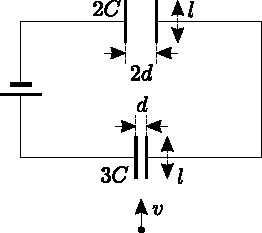
\includegraphics[width=0.6\linewidth]{2005-v3g-08-yl}
\end{center}

\hint
Kondensaatorid on pingeallikaga ühedatud jadamisi ning kondensaatorite $C_1$ ja $C_2$ kogutakistus jadamisi on $\left( 1/C_1 + 1/C_2 \right) ^{-1}$. 

Kuna osakesele mõjuvad elektrijõud on esialgse liikumissuunaga risti, kulub mõlema kondensaatori läbimiseks sama aeg, kusjuures kondensaatorite vahel mõjub osakesele konstantne kiirendus.

\solu
Tegu on kondensaatorite jadaühendusega, mille tõttu laeng mõlemal kondensaatoril peab olema ühesugune. Kondensaatorite kogumahtuvuse leiame valemist 
\[
\frac{1}{C_{0}}=\frac{1}{C_{1}}+\frac{1}{C_{2}} \quad \Rightarrow \quad C_{0}=\num{1,2} C.
\]
Seega laeng on $q = \num{1,2}CU$. Pinge kondensaatoril mahtuvusega $2C$ on seega $U_1 = q/C_1 = \num{0,6}U$ ning kondensaatoril mahtuvusega $3C$ vastavalt $U_2 = \num{0,4}U$. Eeldame, et elektriväli on vaid kondensaatorite sees. Elektrivälja tugevus neis on nüüd vastavalt
\[
E_{1}=-\frac{U_{1}}{2 d}=\frac{-0,3 U}{d} \quad \text { ja } \quad E_{2}=\frac{U_{2}}{d}=\frac{0,4 U}{d}.
\]
Kuna elektriväljad peavad olema suunatud vastupidistes suundades, siis ühe elektrivälja tugevuse võtsime negatiivseks. Määrame nüüd horisontaalsuunalise kiirenduse seosest $Eq = ma$. Esimese kondensaatori puhul on see
\[
a_{2}=\frac{E_{2} q}{m}=\frac{\num{0,4} U q}{m d}.
\]
Vertikaalsuunaline kiirus on kogu aeg sama, selle tõttu aeg, mille jooksul asub osake mõlema kondensaatori elektrivälja mõjusfääris, on $t = l/v$. Selle aja jooksul muutub horisontaalsuunaline kiirus $at$ võrra. Seega teisest kondensaatorist väljumise hetkel on osakese kiirus
\[
v_{h}=t a_{1}+t a_{2}=t\left(a_{1}+a_{2}\right)=\frac{\num{0,1} U q l}{m d v}.
\]
Trajektoori kaldenurga tangens on järelikult
\[
\tan \alpha = \frac{v_h}{v} = \frac{\num{0,1}Uql}{mdv^2}.
\]
\probend